% !TeX root=../main.tex

\chapter{پاسخ سوالات سری دوم}

% دستور زیر باعث عدم‌نمایش شماره صفحه در اولین صفحهٔ این فصل می‌شود.
%\thispagestyle{empty}
\section{پاسخ سوال 1 - الف}

\subsection{پاسخ بخش اول}
در این بخش، از آنجا که تنها موقعیت نهایی ابزار مورد نیاز است و جهت یابی آن خواسته نشده است، می توانیم با استفاده از معادله ی (61.2) موقعیت نهایی را به دست آوریم

\[
\mathbf{A}_{\mathbf{P}} = \mathbf{A}_{\mathbf{P}_{O_B}} + \mathbf{A}_{\mathbf{R}_{B}} \cdot \mathbf{B}_{\mathbf{P}}
\]

برای این منظور، با تقسیم معادلات به دو بخش نوک ابزار و نقطه ی A و ترکیب این دو، می توانیم در نهایت موقعیت نوک ابزار را نسبت به مبدا مختصات به دست آوریم.
در بخش اول که مربوط به پیدا کردن مختصات نقطه ی A در مختصات مبدا است، ابتدا ماتریس دوران حول محور ثابت Z به اندازه ی $\theta$ و ماتریس دوران حول محور متغیر y به اندازه ی $\phi$ را تعریف می کنیم.

\[
R_y(\theta) = \begin{bmatrix}
	\cos(\theta) & 0 & \sin(\theta) \\
	0 & 1 & 0 \\
	-\sin(\theta) & 0 & \cos(\theta)
\end{bmatrix}
\]

\[
R_z(\phi) = \begin{bmatrix}
	\cos(\phi) & -\sin(\phi) & 0 \\
	\sin(\phi) & \cos(\phi) & 0 \\
	0 & 0 & 1
\end{bmatrix}
\]

با در اختیار داشتن ماتریس های دوران، می توانیم با ضرب آن  در موقعیت ابتدایی نقطه ی A، موقعیت جدید نقطه ی A را به دست بیاوریم.

\[
A_0 =
\begin{pmatrix}
	0 \\
	0 \\
	L_{1234}
\end{pmatrix}
\]

\[
P_A = 
\begin{pmatrix}
	L_{1234} \cos(\phi) \sin(\theta) \\
	L_{1234} \sin(\phi) \sin(\theta) \\
	L_{1234} \cos(\theta)
\end{pmatrix}
\]

در اینجا باید توجه شود که چون دوران حول محور z، دوران حول محور متغیر است، بنابراین این ماتریس از سمت چپ ضرب شده است
\subsection{پاسخ بخش دوم}
در بخش بعد، مانند آنچه که در این بخش انجام شدتلاش می شود موقعیت 
نوک ابزار ربات جراح نسبت به موقعیت جدید نقطه ی A به دست می آید.

برای تعریف ماتریس های دوران مربوط به این بخش خواهیم داشت:
\[
R_y(\theta_d) = \begin{bmatrix}
	\cos(\theta_d) & 0 & \sin(\theta_d) \\
	0 & 1 & 0 \\
	-\sin(\theta_d) & 0 & \cos(\theta_d)
\end{bmatrix}
\]

\[
R_z(\phi_d) = \begin{bmatrix}
	\cos(\phi_d) & -\sin(\phi_d) & 0 \\
	\sin(\phi_d) & \cos(\phi_d) & 0 \\
	0 & 0 & 1
\end{bmatrix}
\]

\[
R_y(\alpha + \psi) = \begin{bmatrix}
	\cos(\alpha + \psi) & 0 & \sin(\alpha + \psi) \\
	0 & 1 & 0 \\
	-\sin(\alpha + \psi) & 0 & \cos(\alpha + \psi)
\end{bmatrix}
\]
از ضرب این ماتریس ها با رعایت قاعده ی ضرب از سمت چپ برای دوران های حول محور متحرک در موقعیت اولیه ی نقطه ی ابزار نسبت به نقطه ی A خواهیم داشت:
\[
R_2 = R_y(\alpha + \psi) \cdot R_z(\phi_d) \cdot R_y(\theta_d)
\]
\[
\tiny
R_2 = 
\begin{pmatrix}
	\cos(\alpha + \psi) \cos(\phi_d) \cos(\theta_d) - \sin(\alpha + \psi) \sin(\theta_d) & -\cos(\alpha + \psi) \sin(\phi_d) & \sin(\alpha + \psi) \cos(\theta_d) + \cos(\alpha + \psi) \cos(\phi_d) \sin(\theta_d) \\
	\cos(\theta_d) \sin(\phi_d) & \cos(\phi_d) & \sin(\phi_d) \sin(\theta_d) \\
	-\cos(\alpha + \psi) \sin(\theta_d) - \sin(\alpha + \psi) \cos(\phi_d) \cos(\theta_d) & \sin(\alpha + \psi) \sin(\phi_d) & \cos(\alpha + \psi) \cos(\theta_d) - \sin(\alpha + \psi) \cos(\phi_d) \sin(\theta_d)
\end{pmatrix}
\]
\[
\textbf{d} = 
\begin{pmatrix}
	0 \\
	0 \\
	d
\end{pmatrix}
\]
\[
A_{P_D} = R_2 \cdot \textbf{d} = 
\begin{pmatrix}
	d \left(\sin(\alpha + \psi) \cos(\theta_d) + \cos(\alpha + \psi) \cos(\phi_d) \sin(\theta_d)\right) \\
	d \sin(\phi_d) \sin(\theta_d) \\
	d \left(\cos(\alpha + \psi) \cos(\theta_d) - \sin(\alpha + \psi) \cos(\phi_d) \sin(\theta_d)\right)
\end{pmatrix}
\]
در نهایت پس از به دست آوردن مختصات نقطه ی A نسبت به مرجع و مختصات نقطه ی ابزار نسبت به A، می توانیم مختصات خالص ابزار به مرجع را با استفاده از جمع این دو بردار به دست بیاوریم:

\[
\small
O_P = A_{P_D} + O_{P_A} = 
\begin{pmatrix}
	d \left(\sin(\alpha + \psi) \cos(\theta_d) + \cos(\alpha + \psi) \cos(\phi_d) \sin(\theta_d)\right) + L_{1234} \cos(\phi) \sin(\theta) \\
	L_{1234} \sin(\phi) \sin(\theta) + d \sin(\phi_d) \sin(\theta_d) \\
	L_{1234} \cos(\theta) + d \left(\cos(\alpha + \psi) \cos(\theta_d) - \sin(\alpha + \psi) \cos(\phi_d) \sin(\theta_d)\right)
\end{pmatrix}
\]

برای محاسبات فوق که به صورت نمادین در متلب انجام شده اند، قابلیت جایگذاری عددی برای پارامترهای مورد استفاده نیز طراحی شده است تا بتوان با استفاده از داده های عددی، موقعیت دقیق ابزار را نیز محاسبه کرد.

همچنین، با مراجعه به مقاله ی مربوط به ربات جراح چشم آرش در \cite{hassani2021kinematic} مشاهده می شود که روابط مورد استفاده برای تعیین موقعیت ابزار این ربات به صورت زیر تعریف شده است که تفاوت هایی با مقادیر به دست آمده به روش بالا دارد:
\[
O_P = 
\begin{pmatrix}
	d \left( \sin(\alpha + \psi) \cos(\theta) \cos(\phi) + \cos(\alpha + \psi) \sin(\theta) \cos(\psi) \right) + L_{1234} \sin(\theta) \\
	d \sin(\phi) \sin(\psi + \alpha) \\
	d \left( -\sin(\theta) \cos(\phi) \sin(\psi + \alpha) + \cos(\theta) \cos(\psi + \alpha) \right) + L_{1234} \cos(\theta)
\end{pmatrix}
\]


\section{ پاسخ سوال 2}
\subsection{حل به روش بستار حلقه}

در این روش حل، با در نظر گرفتن مختصات ابزار ربات نسبت به مبدا مختصات O، یک بار به صورت مستقیم و با نام گذاری های 
\[
[x_e, y_e, \theta_e]
\]
 و یک بار نیز با در نظر گرفتن هر یک از مفصل ها و در نهایت با برابر قرار دادن مقادیر به دست آمده از این دو روش، مختصات نهایی را پیدا می کنیم.
 برای این منظور خواهیم داشت:
 \[
 x_e = d_1 + a_3 \cos(\theta_2 + \theta_3) + a_2 \cos(\theta_2)
 \]
 \[
 y_e = a_3 \sin(\theta_2 + \theta_3) + a_2 \sin(\theta_2)
 \]
 \[
 \theta_e = \theta_2 + \theta_3
 \]
 
 \subsubsection{حل به روش دناویت هارتنبرگ}
 برای حل این مسئله به روش دناویت هارتنبرگ، لازم است ابتدا پارامتر های دناویت هارتنبرگ برای هر یک از مفصل ها مشخص شده و در ادامه، با پیاده سازی برنامه ی نرم افزاری و اجرای آن، مختصات نقطه حاصل از تبدیل به دست آمده مخاسبه شود. برای اجرای نرم افزاری، از تابع موجود در پایگاه گیت هاب این درس استفاده شده است.

از آنجا که مفصل اول از نوع کشویی است، بنابراین تنها یک پارامتر $d_1$ دارد. دو مفصل چرخشی بعدی، هر یک دارای یک مقدار a و یک زاویه چرخش $\theta$ می باشند. بنابراین، پارامترهای دناویت هارتنبرگ به صورت زیر محاسبه می شود:
\[
T = \left(\begin{array}{cccc}
	1.0\,\cos \left(\theta_2 +\theta_3 \right) & -1.0\,\sin \left(\theta_2 +\theta_3 \right) & 0 & 1.0\,a_3 \,\cos \left(\theta_2 +\theta_3 \right)+1.0\,a_2 \,\cos \left(\theta_2 \right)\\
	1.0\,\sin \left(\theta_2 +\theta_3 \right) & 1.0\,\cos \left(\theta_2 +\theta_3 \right) & 0 & 1.0\,a_3 \,\sin \left(\theta_2 +\theta_3 \right)+1.0\,a_2 \,\sin \left(\theta_2 \right)\\
	0 & 0 & 1.0 & 1.0\,d_1 \\
	0 & 0 & 0 & 1.0
\end{array}\right)
\]

مشاهده می شود که مقادیر به دست آمده برای $x_e$ و $y_e$ به طور مشخص با نتایج به دست آمده از روش بستار حلقه مطابقت دارند. 
همچنین برای محاسبه ی زاویه ی $\theta$ مطابق رابطه ی زیر خواهیم داشت:
\[
\theta = \arccos\left(\frac{\text{trace}_A - 1}{2}\right)  % \text{Symbolic } \theta \text{ result}
\]
\[
\theta = \frac{180\,\mathrm{acos}\left(1.0\,\cos \left(\theta_2 +\theta_3 \right)\right)}{\pi }
\]
مشخص است که با ساده سازی این عبارت، به جواب به دست آمده در قسمت پیشین خواهیم رسید.

 \subsubsection{حل به روش پیچه های متوالی}

برای حل این سوال به روش پیچه های متوالی، ابتدا محور های مختصات مبدا و ابزار تعیین می شوند. جهت های مورد استفاده در این سوال برای مبدا و نقطه ی انتهایی مطابق با مختصات موجود در کتاب می باشد.
در گام بعد، لازم است محور های پیچه را مشخص کنیم.
بردار پیچه ی اول در راستای محور x، و محور های پیچه ی دوم و سوم در راستای محور z قرار می گیرند. با در نظر گرفتن فواصل، پارامتر های پیچه برای این سوال به صورت زیر به دست می آید:

\begin{table}[h!]
	\centering
	\renewcommand{\arraystretch}{1.5}
	\begin{tabular}{|c|c|c|c|c|c|c|c|c|}
		\hline
		Transformation & \( s_x \) & \( s_y \) & \( s_z \) & \( s_{ox} \) & \( s_{oy} \) & \( s_{oz} \) & \( \theta \) & 0 \\ \hline
		\( S_1 \) & 1 & 0 & 0 & 0 & 0 & 0 & 0 & \( d_1 \) \\ \hline
		\( S_2 \) & 0 & 0 & 1 & 0 & 0 & \( a_1 \) & \( \theta_2 \) & 0 \\ \hline
		\( S_3 \) & 0 & 0 & 1 & 0 & \( a_2 + a_3 \) & 0 & \( \theta_3 \) & 0 \\ \hline
	\end{tabular}
	\caption{Screw Transformation Parameters}
\end{table}
 
 با محاسبه ی ماتریس های تبدیل پیچه و ضرب آنها خواهیم داشت:
 \[
 \tiny
 S = S_1 \times S_2 \times S_3 = 
 \left(\begin{array}{cccc}
 	\cos \left(\theta_2 +\theta_3 \right) & -\sin \left(\theta_2 +\theta_3 \right) & 0 & d_1 +{\left(a_2 +d_1 \right)}\,{\left(\sin \left(\theta_2 +\theta_3 \right)-\sin \left(\theta_2 \right)\right)}\\
 	\sin \left(\theta_2 +\theta_3 \right) & \cos \left(\theta_2 +\theta_3 \right) & 0 & -{\left(a_2 +d_1 \right)}\,{\left(\cos \left(\theta_2 +\theta_3 \right)-\cos \left(\theta_2 \right)\right)}\\
 	0 & 0 & 1 & 0\\
 	0 & 0 & 0 & 1
 \end{array}\right)
 \]
 
 در گام بعد، موقعیت و مختصات ابتدایی و انتهایی نقطه ابزار و مرجع مشخص می شوند:
 \[
 S_0 = 
 \begin{bmatrix}
 	1 & 0 & 0 & a_2 + a_3 \\
 	0 & 1 & 0 & 0 \\
 	0 & 0 & 1 & 0 \\
 	0 & 0 & 0 & 1
 \end{bmatrix}
 \]
 \[
 \tiny
 S_{\text{final}} = 
 \begin{bmatrix}
 	\cos(\theta_2 + \theta_3) & -\sin(\theta_2 + \theta_3) & 0 & d_1 + \cos(\theta_2 + \theta_3)(a_2 + a_3) - a_1 (\cos(\theta_2) - 1) + \sin(\theta_2) \sin(\theta_3)(a_1 + a_2) - \cos(\theta_2)(a_1 + a_2)(\cos(\theta_3) - 1) \\
 	\sin(\theta_2 + \theta_3) & \cos(\theta_2 + \theta_3) & 0 & \sin(\theta_2 + \theta_3)(a_2 + a_3) - a_1 \sin(\theta_2) - \cos(\theta_2) \sin(\theta_3)(a_1 + a_2) - \sin(\theta_2)(a_1 + a_2)(\cos(\theta_3) - 1) \\
 	0 & 0 & 1 & 0 \\
 	0 & 0 & 0 & 1
 \end{bmatrix}
 \]
 
 \[
 \text{Error} = 
 \begin{bmatrix}
 	0 & 0 & 0 & a_1 + d_1 - a_1 \cos(\theta_2 + \theta_3) \\
 	0 & 0 & 0 & -a_1 \sin(\theta_2 + \theta_3) \\
 	0 & 0 & 0 & -d_1 \\
 	0 & 0 & 0 & 0
 \end{bmatrix}
 \]
 
 با مقایسه ی این ماتریس با نتایج بخش های قبل مشاهده می شود که ماتریس دوران حاصل از روش پیچه به درستی محاسبه شده است اما تفاوت هایی در ماتریس انتقال وجود دارد.

 \subsubsection{فضای کاری ربات}
 
 با در اختیار داشتن ماتریس دوران و تعیین اندازه ی طول بازوهای ربات، می توانیم به ازای مقادیر مشخص برای زوایای چرخش بازوها و میزان جابه جایی بازوی اول به صورت زیر به دست می آید:
 
 
\begin{figure}[H]
	\centering
	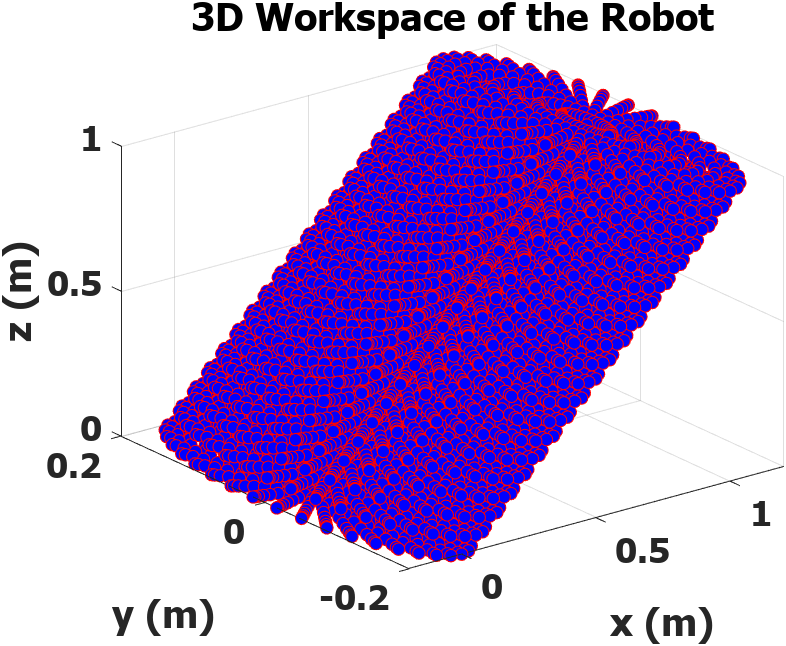
\includegraphics[width=0.7\linewidth]{../img/2_Workspace}
	\caption{}
	\label{fig:2workspace}
\end{figure}
 
\section{ پاسخ سوال 3}
\subsection{روش دناویت هارتنبرگ}

پارامتر های DH ربات Kuka IIWA مطابق با 
\cite{slim2023inverse}
به صورت زیر به دست می آید.
\begin{table}[h!]
	\centering
	\renewcommand{\arraystretch}{1.5}
	\begin{tabular}{|c|c|c|c|c|}
		\hline
		Link & \( a_i \) & \( \alpha_i \) & \( d_i \) & \( \theta_i \) \\ \hline
		1 & 0 & \( -\frac{\pi}{2} \) & \( d_1 \) & \( \theta_1 \) \\ \hline
		2 & 0 & \( \frac{\pi}{2} \) & 0 & \( \theta_2 \) \\ \hline
		3 & 0 & \( \frac{\pi}{2} \) & \( d_3 \) & \( \theta_3 \) \\ \hline
		4 & 0 & \( -\frac{\pi}{2} \) & 0 & \( \theta_4 \) \\ \hline
		5 & 0 & \( -\frac{\pi}{2} \) & \( d_5 \) & \( \theta_5 \) \\ \hline
		6 & 0 & \( \frac{\pi}{2} \) & 0 & \( \theta_6 \) \\ \hline
		7 & 0 & 0 & \( d_7 \) & \( \theta_7 \) \\ \hline
	\end{tabular}
	\caption{پارامتر های DH ربات Kuka IIWA}
\end{table}

با در اختیار داشتن این تبدیل ها و استفاده از تابع نوشته شده برای محاسبه ی ماتریس تبدیل حاصل از هر یک از این تبدیل ها و با ضرب متوالی آنها، در نهایت پس از ساده سازی خواهیم داشت:

\[
T = \begin{pmatrix}
	T_{11} & T_{12} & T_{13} & T_{14} \\
	T_{21} & T_{22} & T_{23} & T_{24} \\
	T_{31} & T_{32} & T_{33} & T_{34} \\
	T_{41} & T_{42} & T_{43} & T_{44} \\
\end{pmatrix}
\]

به دلیل محدودیت در فضای گزارش، المان های این ماتریس به در این قسمت آورده نشده است، اما با مراجعه به کد متلب مربوطه، می توان این ماتریس را مشاهده کرد.

\subsection{روش پیچه های متوالی}
برای حل این مسئله به روش پیچه های متوالی، به طریق زیر عمل می کنیم.
ابتدا دستگاه های مختصات مرجع و ابزار را بر روی ربات قرار می دهیم. جهت گیری این محور ها مطابق با شکل رسم شده در کتاب می باشد.
در گام بعد، موقعیت و جهت گیری اولیه ی ابزار ربات را به صورت زیر به دست می آوریم:

\[
x_e^0 = \begin{bmatrix}
	0 \\
	0 \\
	a_1 + a_3 + a_5 + a_7
\end{bmatrix}
\]
\[
R_e^0 = \begin{bmatrix}
	1 & 0 & 0 \\
	0 & 1 & 0 \\
	0 & 0 & 1
\end{bmatrix}
\]
در اینجا مشاهده می شود که در وضعیت ابتدایی، جهت گیری ابزار نسبت به وضعیت مرجع تغییری ندارد و تنها موقعیت آن به اندازه ی طول بازوهای ربات جابه جا شده است.
در گام بعد، محور های پیچه باید تعریف شوند.
اما پارامتر های در نظر گرفته شده، مربوط به تمام بازوهای ربات هستند. دراین بخش، به منظور سادگی ابتدا تنها به بررسی سه درجه اول ربات می پردازیم و در بخش های بعد، 2 درجه ی دوم و سوم مورد بررسی قرار می گیرد.
\subsubsection{3 درجه اول}

در اینجا خواهیم داشت:
\[
x_3^0 = \begin{bmatrix}
	0 \\
	0 \\
	a_1 + a_3
\end{bmatrix}
\]
\[
R_3^0 = \begin{bmatrix}
	1 & 0 & 0 \\
	0 & 1 & 0 \\
	0 & 0 & 1
\end{bmatrix}
\]
 مجددا با توجه به جهتگیری دستگاه ها، مشاهده می شود که تغییری در جهت گیری نداریم. 
 حال، لازم است پارامتر های پیچه برای این تبدیل ها مشخص شوند.
 بنابراین خواهیم داشت:
\[
S_1 = SR(0, 0, 1, 0, 0, 0, \theta_1, 0) \quad \text{(پیچه 1)}
\]
\[
S_2 = SR(0, 1, 0, 0, 0, a_1, \theta_2, 0) \quad \text{(پیچه 2)}
\]
\[
S_3 = SR(0, 0, 1, 0, 0, 0, \theta_3, 0) \quad \text{(پیچه 3)}
\]

سه پارامتر اول، با مقایسه ی جهت هر یک از محور های دستگاه بعدی در مقایسه با دستگاه مرجع انتخاب شده اند.  همچنین، مقدار a با در نظر گرفتن فاصله ی دستگاه مورد نظر تا مرجع به دست آمده است.

ماتریس تبدیل حاصل از این سه حرکت، از ضرب و ساده سازی سه ماتریس بالا به صورت زیر به دست می آید.
\[
\tiny
S_1 \cdot S_2 \cdot S_3 =
\left(\begin{array}{cccc}
	\cos \left(\theta_1 \right)\,\cos \left(\theta_2 \right)\,\cos \left(\theta_3 \right)-\sin \left(\theta_1 \right)\,\sin \left(\theta_3 \right) & -\cos \left(\theta_3 \right)\,\sin \left(\theta_1 \right)-\cos \left(\theta_1 \right)\,\cos \left(\theta_2 \right)\,\sin \left(\theta_3 \right) & \cos \left(\theta_1 \right)\,\sin \left(\theta_2 \right) & -a_1 \,\cos \left(\theta_1 \right)\,\sin \left(\theta_2 \right) \\
	\cos \left(\theta_1 \right)\,\sin \left(\theta_3 \right)+\cos \left(\theta_2 \right)\,\cos \left(\theta_3 \right)\,\sin \left(\theta_1 \right) & \cos \left(\theta_1 \right)\,\cos \left(\theta_3 \right)-\cos \left(\theta_2 \right)\,\sin \left(\theta_1 \right)\,\sin \left(\theta_3 \right) & \sin \left(\theta_1 \right)\,\sin \left(\theta_2 \right) & -a_1 \,\sin \left(\theta_1 \right)\,\sin \left(\theta_2 \right) \\
	-\cos \left(\theta_3 \right)\,\sin \left(\theta_2 \right) & \sin \left(\theta_2 \right)\,\sin \left(\theta_3 \right) & \cos \left(\theta_2 \right) & -a_1 \,{\left(\cos \left(\theta_2 \right)-1\right)} \\
	0 & 0 & 0 & 1
\end{array}\right)
\]
سپس با مشخص کردن ماتریس تبدیل نقطه ی اولیه به نقطه ی ثانویه به صورت زیر خواهیم داشت:
 حال با پیاده سازی	معادلات DH مطابق پارامتر های زیر خواهیم داشت:
 \[
 T_1 = DH(0, -\frac{\pi}{2}, a_1, \theta_1) \quad \text{(پارامترهای دناویت هارتنبرگ 1)}
 \]
 \[
 T_2 = DH(0, \frac{\pi}{2}, 0, \theta_2) \quad \text{(پارامترهای دناویت هارتنبرگ 2)}
 \]
 \[
 T_3 = DH(0, \frac{\pi}{2}, a_3, \theta_3) \quad \text{(پارامترهای دناویت هارتنبرگ 3)}
 \]
 
 آنگاه با محاسبه ی ماتریس تبدیل حاصل از این تبدیل ها خواهیم داشت:
 \[
 U_0 = \begin{bmatrix} 1 \\ 0 \\ 0 \end{bmatrix}, \quad
 V_0 = \begin{bmatrix} 0 \\ 1 \\ 0 \end{bmatrix}, \quad
 W_0 = \begin{bmatrix} 0 \\ 0 \\ 1 \end{bmatrix}, \quad
 E_0 = \begin{bmatrix} 0 \\ 0 \\ a_1 + a_3 \end{bmatrix}
 \]
 
 \[
 S_0 = \begin{bmatrix}
 	U_0 & V_0 & W_0 & E_0 \\
 	0 & 0 & 0 & 1
 \end{bmatrix} = 
 \begin{bmatrix}
 	1 & 0 & 0 & 0 \\
 	0 & 1 & 0 & 0 \\
 	0 & 0 & 1 & a_1 + a_3 \\
 	0 & 0 & 0 & 1
 \end{bmatrix}
 \]
 سپس، با ضرب ماتریس تبدیل به دست آمده در این ماتریس، موقعیت و جهت گیری نقطه ی انتهایی بازوی سوم مشخص می شود:
 \[
 \tiny
 S_3^0 = 
 \begin{bmatrix}
 	\cos \left(\theta_1 \right)\,\cos \left(\theta_2 \right)\,\cos \left(\theta_3 \right) - \sin \left(\theta_1 \right)\,\sin \left(\theta_3 \right) & -\cos \left(\theta_3 \right)\,\sin \left(\theta_1 \right) - \cos \left(\theta_1 \right)\,\cos \left(\theta_2 \right)\,\sin \left(\theta_3 \right) & \cos \left(\theta_1 \right)\,\sin \left(\theta_2 \right) & \cos \left(\theta_1 \right)\,\sin \left(\theta_2 \right)\,(a_1 + a_3) - a_1 \,\cos \left(\theta_1 \right)\,\sin \left(\theta_2 \right) \\
 	\cos \left(\theta_1 \right)\,\sin \left(\theta_3 \right) + \cos \left(\theta_2 \right)\,\cos \left(\theta_3 \right)\,\sin \left(\theta_1 \right) & \cos \left(\theta_1 \right)\,\cos \left(\theta_3 \right) - \cos \left(\theta_2 \right)\,\sin \left(\theta_1 \right)\,\sin \left(\theta_3 \right) & \sin \left(\theta_1 \right)\,\sin \left(\theta_2 \right) & \sin \left(\theta_1 \right)\,\sin \left(\theta_2 \right)\,(a_1 + a_3) - a_1 \,\sin \left(\theta_1 \right)\,\sin \left(\theta_2 \right) \\
 	-\cos \left(\theta_3 \right)\,\sin \left(\theta_2 \right) & \sin \left(\theta_2 \right)\,\sin \left(\theta_3 \right) & \cos \left(\theta_2 \right) & \cos \left(\theta_2 \right)\,(a_1 + a_3) - a_1 \,(\cos \left(\theta_2 \right) - 1) \\
 	0 & 0 & 0 & 1
 \end{bmatrix}
 \]
 
در نهایت، مشاهده می شود که مقدار انتقال با نتایج به دست آمده از روش دناویت هارتنبرگ برابر است، اما ماتریس دوران تفاوت دارد.

 


\begin{thebibliography}{9}
	
	\bibitem{hassani2021kinematic}
	A. Hassani, M.R. Dindarloo, R. Khorambakht, A. Bataleblu, H. Sadeghi, R. Heidari, A. Iranfar, P. Hasani, N.S. Hojati, A. Khorasani, et al.,
	\textit{Kinematic and dynamic analysis of arash asist: Toward micro positioning}, 
	in \textit{2021 9th RSI International Conference on Robotics and Mechatronics (ICRoM)}, 
	pp. 59--65, 2021, IEEE.
	
	\bibitem{slim2023inverse}
	Slim, M.; Rokbani, N.; Neji, B.; Terres, M. A.; Beyrouthy, T.
	\newblock Inverse kinematic solver based on bat algorithm for robotic arm path planning.
	\newblock {\em Robotics} \textbf{2023}, {\em 12}(2), 38.
	
\end{thebibliography}

